\documentclass{standalone}
\usepackage{xcolor}
\usepackage{tikz}
\usepackage{pgfplots}
\usetikzlibrary{math}
\usetikzlibrary{calc}
\definecolor{solColor}{rgb}{1,0.5,0}
\definecolor{otherColor}{gray}{0.7}

\begin{document}
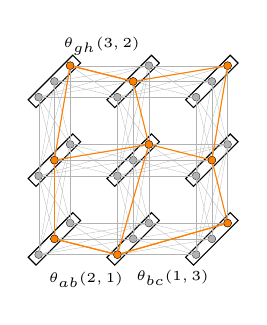
\begin{tikzpicture}
%\foreach \i in {0,...,3} {
%	\draw [very thin, lightgray, dashed] (\i,0) -- (\i,3) node [below] at (\i,0) {};
%}
%\foreach \i in {1,...,3} {
%	\draw [very thin, lightgray, dashed] (1,\i) -- (3,\i) node [left] at (0,\i) {};
%}
\foreach \x in {0,...,2} {
	\foreach \y in {0,...,2} {
		\foreach \l in {0,...,2} {
			\tikzmath{\h = (\l-1)/5;}
			\node[circle,draw=black,ultra thin,fill=otherColor,scale=0.3] (\x-\y-\l) at (\x + \h + 0.5,\y + \h + 0.5) {}; 
		}
			\draw[black,rotate around={45:(\x + 0.5,\y + 0.5)}] (\x+ 0.5-0.40,\y+ 0.5-0.07) rectangle (\x+ 0.5+0.40,\y+0.5+0.07);
	}
}
\foreach \x in {0,...,2} {
	\tikzmath{\xn = \x+1;}
	\foreach \y in {0,...,2} {
		\tikzmath{\yn = \y+1;}
		\foreach \l in {0,...,2} {
			\tikzmath{\hpp = (\l-3)/5;}
			\tikzmath{\hp = (\l-2)/5;}
			\tikzmath{\h = (\l-1)/5;}
			\tikzmath{\hn = (\l)/5;}
			\tikzmath{\hnn = (\l+1)/5;}
			\ifnum \x < 2
				\draw [ultra thin, otherColor] (\x + \h + 0.5,\y + \h + 0.5) -- (\xn + \h + 0.5,\y + \h + 0.5);
				\ifnum \l=0
					\draw [ultra thin, otherColor] (\x + \h + 0.5,\y + \h + 0.5) -- (\xn + \hn + 0.5,\y + \hn + 0.5);
					\draw [ultra thin, otherColor] (\x + \h + 0.5,\y + \h + 0.5) -- (\xn + \hnn + 0.5,\y + \hnn + 0.5);
				\fi
				\ifnum \l=1
					\draw [ultra thin, otherColor] (\x + \h + 0.5,\y + \h + 0.5) -- (\xn + \hp + 0.5,\y + \hp + 0.5);
					\draw [ultra thin, otherColor] (\x + \h + 0.5,\y + \h + 0.5) -- (\xn + \hn + 0.5,\y + \hn + 0.5);
				\fi
				\ifnum \l=2
					\draw [ultra thin, otherColor] (\x + \h + 0.5,\y + \h + 0.5) -- (\xn + \hp + 0.5,\y + \hp + 0.5);
					\draw [ultra thin, otherColor] (\x + \h + 0.5,\y + \h + 0.5) -- (\xn + \hpp + 0.5,\y + \hpp + 0.5);
				\fi 
			\fi
			\ifnum \y < 2
				\draw [ultra thin, otherColor] (\x + \h + 0.5,\y + \h + 0.5) -- (\x + \h + 0.5,\yn + \h + 0.5);
				\ifnum \l=0
				\draw [ultra thin, otherColor] (\x + \h + 0.5,\y + \h + 0.5) -- (\x + \hn + 0.5,\yn + \hn + 0.5);
				\draw [ultra thin, otherColor] (\x + \h + 0.5,\y + \h + 0.5) -- (\x + \hnn + 0.5,\yn + \hnn + 0.5);
				\fi
				\ifnum \l=1
				\draw [ultra thin, otherColor] (\x + \h + 0.5,\y + \h + 0.5) -- (\x + \hp + 0.5,\yn + \hp + 0.5);
				\draw [ultra thin, otherColor] (\x + \h + 0.5,\y + \h + 0.5) -- (\x + \hn + 0.5,\yn + \hn + 0.5);
				\fi
				\ifnum \l=2
				\draw [ultra thin, otherColor] (\x + \h + 0.5,\y + \h + 0.5) -- (\x + \hp + 0.5,\yn + \hp + 0.5);
				\draw [ultra thin, otherColor] (\x + \h + 0.5,\y + \h + 0.5) -- (\x + \hpp + 0.5,\yn + \hpp + 0.5);
				\fi 
			\fi
		}
	}
}
\tikzmath{\hd = (1)/5;}
\node[circle,draw=black,ultra thin,fill=orange,scale=0.3] (x1) at (0.5,0.5) {}; 
\node[circle,draw=black,ultra thin,fill=orange,scale=0.3] (x2) at (1.5-\hd,0.5-\hd) {}; 
\node[circle,draw=black,ultra thin,fill=orange,scale=0.3] (x3) at (2.5+\hd,0.5+\hd) {}; 
\node[circle,draw=black,ultra thin,fill=orange,scale=0.3] (x4) at (0.5,1.5) {}; 
\node[circle,draw=black,ultra thin,fill=orange,scale=0.3] (x5) at (1.5+\hd,1.5+\hd) {}; 
\node[circle,draw=black,ultra thin,fill=orange,scale=0.3] (x6) at (2.5,1.5) {}; 
\node[circle,draw=black,ultra thin,fill=orange,scale=0.3] (x7) at (0.5+\hd,2.5+\hd) {}; 
\node[circle,draw=black,ultra thin,fill=orange,scale=0.3] (x8) at (1.5,2.5) {}; 
\node[circle,draw=black,ultra thin,fill=orange,scale=0.3] (x9) at (2.5+\hd,2.5+\hd) {}; 
\path [draw, orange] (x1) -- (x2) node[midway] (12) {};
\path [draw, orange] (x2) -- (x3) node[midway] (23) {};
\path [draw, orange] (x1) -- (x4) node[midway] (14) {};
\path [draw, orange] (x2) -- (x5) node[midway] (25) {};
\path [draw, orange] (x3) -- (x6) node[midway] (36) {};
\path [draw, orange] (x4) -- (x5) node[midway] (45) {};
\path [draw, orange] (x5) -- (x6) node[midway] (56) {};
\path [draw, orange] (x4) -- (x7) node[midway] (47) {};
\path [draw, orange] (x5) -- (x8) node[midway] (58) {};
\path [draw, orange] (x6) -- (x9) node[midway] (69) {};
\path [draw, orange] (x7) -- (x8) node[midway] (78) {};
\path [draw, orange] (x8) -- (x9) node[midway] (89) {};
%
\node[orange, left of=47, node distance = 6pt] (){};
\node[orange, left of=58, node distance = 6pt] (){};
\node[orange, left of=36, node distance = 6pt] (){};
\node[orange, below of=12, node distance = 6pt] (){};
\path [draw, solColor] (x1) -- (x2) node[midway] (12) {};
\node[solColor, below of=12, node distance = 12pt] (){\tiny \textcolor{black}{$\theta_{ab}(2, 1)$}};
\path [draw, solColor] (x2) -- (x3) node[midway] (23) {};
\node[solColor, below of=23, node distance = 14pt] (){\tiny \textcolor{black}{$\theta_{bc}(1, 3)$}};
\path [draw, solColor] (x7) -- (x8) node[midway] (78) {};
\node[solColor, above of=78, node distance = 10pt] (){\tiny \textcolor{black}{$\theta_{gh}(3, 2)$}};
%
\end{tikzpicture}
\end{document}
